% Source: Code/ML_overlay/ir_rgb_registration/paper/ml_overlay_report_materials/ir_rgb_registration_report/figures/fig_transformer_flow.tex
\documentclass[tikz,border=10pt]{standalone}
\usepackage{tikz}
\usepackage{amsmath}
\usetikzlibrary{positioning,shapes.geometric,arrows.meta,calc,fit}

\definecolor{Garnet}{RGB}{115,0,10}
\definecolor{Rose}{RGB}{204,46,64}
\definecolor{Atlantic}{RGB}{70,106,159}
\definecolor{Congaree}{RGB}{31,65,77}
\definecolor{Horseshoe}{RGB}{101,120,11}
\definecolor{Honeycomb}{RGB}{164,145,55}
\definecolor{Black90}{RGB}{54,54,54}
\definecolor{Black70}{RGB}{92,92,92}

\begin{document}
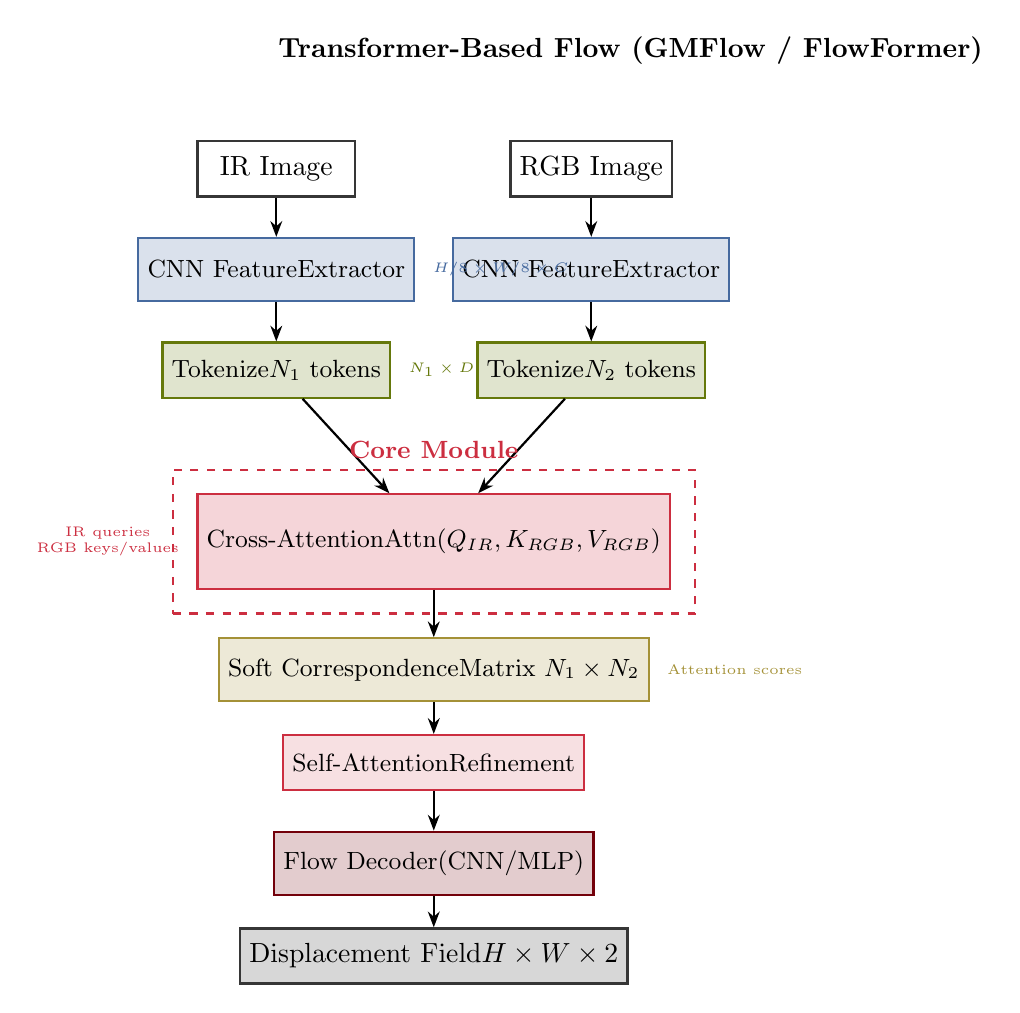
\begin{tikzpicture}[
    encoder/.style={rectangle,draw=Atlantic,fill=Atlantic!20,thick,minimum width=2cm,minimum height=0.8cm,font=\small},
    token/.style={rectangle,draw=Horseshoe,fill=Horseshoe!20,thick,minimum width=2cm,minimum height=0.7cm,font=\small},
    attention/.style={rectangle,draw=Rose,fill=Rose!20,thick,minimum width=3cm,minimum height=1.2cm,font=\small},
    corr/.style={rectangle,draw=Honeycomb,fill=Honeycomb!20,thick,minimum width=2.5cm,minimum height=0.8cm,font=\small},
    decoder/.style={rectangle,draw=Garnet,fill=Garnet!20,thick,minimum width=2cm,minimum height=0.8cm,font=\small},
    arrow/.style={-{Stealth[length=2mm]},thick}
]

\node[font=\bfseries] at (6,10.5) {Transformer-Based Flow (GMFlow / FlowFormer)};

% Input images
\node[rectangle,draw=Black90,thick,minimum width=2cm,minimum height=0.7cm] (ir-input) at (1.5,9) {IR Image};
\node[rectangle,draw=Black90,thick,minimum width=2cm,minimum height=0.7cm] (rgb-input) at (5.5,9) {RGB Image};

% Feature extractors
\node[encoder,below=0.5cm of ir-input] (ir-feat) {CNN Feature\\Extractor};
\node[encoder,below=0.5cm of rgb-input] (rgb-feat) {CNN Feature\\Extractor};

\draw[arrow] (ir-input) -- (ir-feat);
\draw[arrow] (rgb-input) -- (rgb-feat);

% Tokenization
\node[token,below=0.5cm of ir-feat] (ir-token) {Tokenize\\$N_1$ tokens};
\node[token,below=0.5cm of rgb-feat] (rgb-token) {Tokenize\\$N_2$ tokens};

\draw[arrow] (ir-feat) -- (ir-token);
\draw[arrow] (rgb-feat) -- (rgb-token);

% Cross-attention block (highlighted)
\node[attention,below=1.2cm of rgb-token,xshift=-2cm] (cross-attn) {Cross-Attention\\$\text{Attn}(Q_{IR}, K_{RGB}, V_{RGB})$};

\draw[arrow] (ir-token) -- (cross-attn);
\draw[arrow] (rgb-token) -- (cross-attn);

% Highlight box around cross-attention
\node[draw=Rose,thick,dashed,fit=(cross-attn),inner sep=0.3cm,label={[Rose,font=\small\bfseries]above:Core Module}] {};

% Correspondence matrix
\node[corr,below=0.6cm of cross-attn] (corr-mat) {Soft Correspondence\\Matrix $N_1 \times N_2$};

\draw[arrow] (cross-attn) -- (corr-mat);

% Self-attention refinement
\node[rectangle,draw=Rose,fill=Rose!15,thick,minimum width=2.5cm,minimum height=0.7cm,font=\small,below=0.4cm of corr-mat] (self-attn) {Self-Attention\\Refinement};

\draw[arrow] (corr-mat) -- (self-attn);

% Decoder
\node[decoder,below=0.5cm of self-attn] (decoder-block) {Flow Decoder\\(CNN/MLP)};

\draw[arrow] (self-attn) -- (decoder-block);

% Displacement field output
\node[rectangle,draw=Black90,fill=Black90!20,thick,minimum width=2.5cm,minimum height=0.7cm,below=0.4cm of decoder-block] (output) {Displacement Field\\$H \times W \times 2$};

\draw[arrow] (decoder-block) -- (output);

% Annotations
\node[font=\tiny,text=Atlantic,right=0.1cm of ir-feat] {$H/8 \times W/8 \times C$};
\node[font=\tiny,text=Horseshoe,right=0.1cm of ir-token] {$N_1 \times D$};
\node[font=\tiny,text=Honeycomb,right=0.1cm of corr-mat] {Attention scores};

% Add bidirectional annotation for cross-attention
\node[font=\tiny,text=Rose,left=0.1cm of cross-attn,align=center] {IR queries\\RGB keys/values};

\end{tikzpicture}
\end{document}
